% Two-page roadmap handout for students (A4)
\documentclass[10.5pt,a4paper]{article}
\usepackage[T1]{fontenc}
\usepackage{lmodern}
\usepackage[margin=1.7cm, top=1.5cm]{geometry}
\usepackage{booktabs, tabularx, array, xcolor, tikz, enumitem, multicol, hyperref}
\usetikzlibrary{arrows.meta, positioning}
\definecolor{ocean}{HTML}{0D366B}\definecolor{sea}{HTML}{2A78D6}\definecolor{coral}{HTML}{EB6834}
\definecolor{kelp}{HTML}{1BAF7A}\definecolor{muted}{HTML}{52514E}
\hypersetup{colorlinks, urlcolor=sea, linkcolor=ocean}
\setlist{nosep, leftmargin=1.2em}
\pagestyle{empty}
\setlength{\parindent}{0pt}
\newcommand{\sect}[1]{\par\medskip{\color{ocean}\large\bfseries #1}\par\smallskip}
\begin{document}
{\color{ocean}\Huge\bfseries Can a computer identify deep-sea animals?}\\[3pt]
{\large A hands-on classifier project with FathomNet 2025 \quad\textcolor{muted}{$\cdot$ Roadmap for students}}
\par\medskip
\textcolor{coral}{\rule{\linewidth}{1.2pt}}

\begin{multicols}{2}
\sect{What this project is}
Deep-sea video produces far more animals than experts can name. You will teach a computer to name them:
you build \textbf{classifiers} -- rules that turn a picture into a label -- from 23{,}698 expert-labelled
crops of 79 deep-sea animals (FathomNet 2025), compare them, and find out \textbf{when they can be trusted}.

\sect{What you need}
A Google account (Colab) or Python on your laptop. No programming experience: the notebooks are ready, you change
a word or a number. No GPU.

\sect{What you will be able to do}
\begin{itemize}
\item explain classifier, feature, training/test set, overfitting
\item use six classifiers and three kinds of features
\item read accuracy, recall, precision, a confusion matrix
\item judge mistakes with the tree of life
\item decide whether a classifier is fit for a survey
\end{itemize}
\columnbreak
\sect{Words to know}
\small
\begin{tabularx}{\linewidth}{@{}>{\bfseries}lX@{}}
crop & the cut-out picture of one animal \\
label & the name an expert gave it (79 labels) \\
feature & a number describing the crop (a character) \\
classifier & rule: features $\to$ label, learned from examples \\
training set & examples the rule is learned from \\
test set & other examples, only for grading \\
validation set & examples for choosing between ideas \\
overfitting & learning the examples by heart \\
baseline & always guess the most common label \\
dive & one ROV deployment; frames of a dive look alike \\
CNN & neural network for images; gives 512 features \\
\end{tabularx}
\end{multicols}

\sect{The roadmap}
\begin{center}
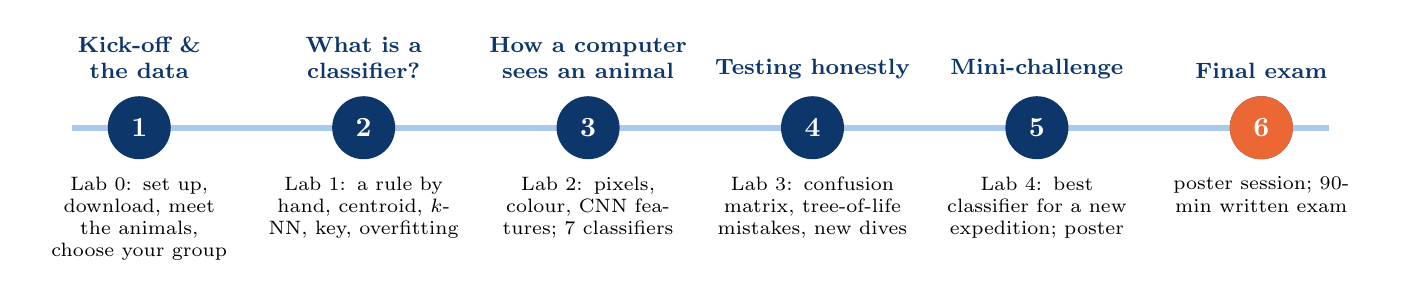
\begin{tikzpicture}[x=2.85cm, >=Stealth,
  wk/.style={circle, fill=ocean, text=white, font=\bfseries, minimum size=8mm, inner sep=0},
  lab/.style={text width=25mm, align=center, font=\scriptsize, anchor=north},
  ttl/.style={text width=26mm, align=center, font=\footnotesize\bfseries, text=ocean, anchor=south}]
  \draw[line width=2.2pt, sea!40] (0.7,0) -- (6.3,0);
  \foreach \i/\t/\l in {
    1/Kick-off \& the data/{Lab 0: set up, download, meet the animals, choose your group},
    2/What is a classifier?/{Lab 1: a rule by hand, centroid, $k$-NN, key, overfitting},
    3/How a computer sees an animal/{Lab 2: pixels, colour, CNN features; 7 classifiers},
    4/Testing honestly/{Lab 3: confusion matrix, tree-of-life mistakes, new dives},
    5/Mini-challenge/{Lab 4: best classifier for a new expedition; poster},
    6/Final exam/{poster session; 90-min written exam}} {
    \node[wk] at (\i,0) {\i};
    \node[ttl] at (\i,0.5) {\t};
    \node[lab] at (\i,-0.5) {\l};
  }
  \node[wk, fill=coral] at (6,0) {6};
\end{tikzpicture}
\end{center}

\small
\begin{tabularx}{\linewidth}{@{}c>{\raggedright}p{3.3cm}>{\raggedright\ttfamily\arraybackslash}p{4.1cm}X@{}}
\toprule
& \textbf{Session} & \textbf{\normalfont Notebook} & \textbf{Hand in (by the next session)} \\
\midrule
1 & Kick-off \& the data & lab0\_data & your group, its labels, one figure; Q1--Q5 \\
2 & What is a classifier? & lab1\_first\_classifier & your threshold and key; Q1--Q4 \\
3 & How a computer sees an animal & lab2\_features\_and\_zoo & results table; Q1--Q5 \\
4 & Testing honestly & lab3\_honest\_evaluation & confusion matrix, split chart, half page; Q1--Q7 \\
5 & Mini-challenge & lab4\_challenge & leaderboard entry; poster (A3 or 4 slides) \\
6 & Poster session \& exam & -- & -- \\
\bottomrule
\end{tabularx}

\normalsize
\begin{multicols}{2}
\sect{How to start}
\begin{enumerate}
\item Open \texttt{course/lab0\_data.ipynb} in Google Colab (File $\to$ Upload notebook) or in Jupyter.
\item Run the first cell. It downloads the course and the crops (about 15 min the first time; a copy is kept on your Google Drive).
\item Run the cells in order (\emph{Shift+Enter}). Answer the \textbf{\color{coral}\ Q} cells in the notebook.
\item Hand in the notebook (File $\to$ Download .ipynb).
\end{enumerate}
\columnbreak
\sect{Grading (suggested)}
\begin{tabularx}{\linewidth}{@{}Xr@{}}
\toprule
Lab notebooks 0--3 (answers to Q cells) & 30\,\% \\
Mini-challenge poster (+ small leaderboard bonus) & 30\,\% \\
Final exam (90 min, written, no code) & 40\,\% \\
\bottomrule
\end{tabularx}

\sect{Rules}
Work in pairs. Never tune on the test set. Acknowledge \textbf{FathomNet and MBARI} on your poster
(images CC BY-NC-ND 4.0). Do not re-download the data in a loop -- the servers are shared.
\end{multicols}
\end{document}
